\documentclass[aspectratio=169]{beamer}
\usepackage[utf8]{inputenc}
\usepackage[T1]{fontenc}
\usepackage[italian]{babel}
\usepackage{graphicx}
\usepackage{booktabs}
\usepackage{xcolor}
\usepackage{amsmath}

% Tema Beamer
\usetheme{Madrid}
\usecolortheme{whale}

% Modifiche per renderlo più pulito
\setbeamertemplate{navigation symbols}{}
\setbeamertemplate{footline}[frame number]

\title[Data Drift su ImageNet]{Report progetto Architetture Dati: data drift su ImageNet}
\subtitle{Analisi delle prestazioni di ResNet-50 su ImageNet-R e ImageNet-C}
\author[Besozzi, Consonni, Zen]{Daniele Besozzi 894998, Andrea Consonni 900116, Elena Zen 895355}
\institute{Progetto Architetture Dati}
\date{}

\begin{document}

\begin{frame}
  \titlepage
\end{frame}

\begin{frame}{Indice}
  \tableofcontents[hideallsubsections]
\end{frame}

% --- CAPITOLO 1: INTRODUZIONE ---
\section{Introduzione al Data Drift}

\begin{frame}{Il problema del Data Drift}
    \begin{itemize}
        \item \textbf{Assunzione classica (i.i.d.)}: Nel machine learning si assume che i dati di test e di addestramento provengano dalla stessa distribuzione e che siano indipendenti.
        \item \textbf{Realtà operativa}: Spesso questa assunzione è disattesa. La distribuzione cambia nel tempo o nello spazio $\rightarrow$ \textbf{Data drift} o \textbf{Distribution shift}.
        \item \textbf{Conseguenza}: Calo significativo delle prestazioni del modello, anche senza alcuna modifica ai suoi pesi o all'architettura.
        \item \textbf{Obiettivo del progetto}: Quantificare l'effetto del drift sulle prestazioni dei modelli di classificazione d'immagini.
    \end{itemize}
\end{frame}

\begin{frame}{Definizione Formale}
    Secondo Moreno-Torres et al., possiamo definire il \textbf{Dataset Shift} come:
    \vspace{0.3cm}
    \begin{block}{Dataset shift}
        Si verifica quando la distribuzione di probabilità congiunta delle feature $x$ e della variabile target $y$ differisce tra la fase di addestramento ($P_{tr}$) e la fase di test ($P_{tst}$).\\
        Formalmente: $P_{tr}(y,x) \neq P_{tst}(y,x)$.
    \end{block}
    \vspace{0.3cm}
    È essenziale distinguere la direzione causale:
    \begin{itemize}
        \item $X \rightarrow Y$: Le feature determinano la classe (es. frodi bancarie).
        \item $Y \rightarrow X$: La classe determina le feature (es. patologia che causa sintomi).
    \end{itemize}
\end{frame}

\begin{frame}{Tipologie di Data Drift: Covariate Shift}
    \begin{columns}
        \begin{column}{0.5\textwidth}
            \textbf{Covariate Shift (o Population Drift)}
            \begin{itemize}
                \item Cambiano le feature in input, ma la classe semantica resta la stessa.
                \item $P_{tr}(x) \neq P_{tst}(x)$ e $P_{tr}(y|x) = P_{tst}(y|x)$.
                \item È la forma di drift indagata in questo progetto (variazioni di stile, perturbazioni visive).
            \end{itemize}
        \end{column}
        \begin{column}{0.5\textwidth}
            \centering
            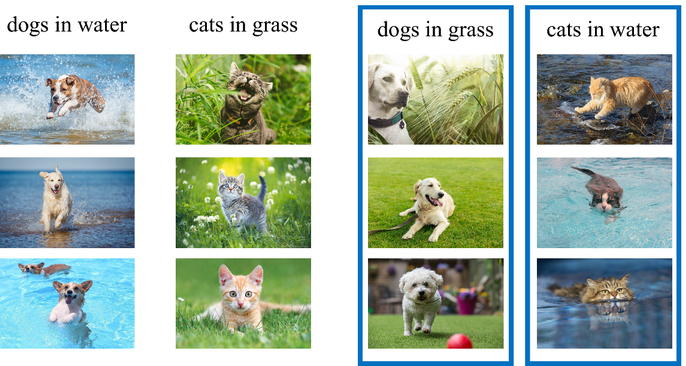
\includegraphics[width=\textwidth,height=0.7\textheight,keepaspectratio]{images/covariate_shift.png}
        \end{column}
    \end{columns}
\end{frame}

\begin{frame}{Altre Tipologie e Cause}
    \begin{block}{Prior Probability Shift}
        Cambia la frequenza delle classi ($P(y)$ fluttua), ma la distribuzione delle feature data la classe resta uguale. Tipico della diagnostica (epidemie).
    \end{block}
    \begin{block}{Concept Shift}
        Cambia la definizione stessa della classe da apprendere ($P_{tr}(y|x) \neq P_{tst}(y|x)$). Esempio: spammer che cambiano tattiche per ingannare i filtri.
    \end{block}
    \vspace{0.3cm}
    \textbf{Cause principali del drift}:
    \begin{itemize}
        \item Sample Selection Bias (campionamento non uniforme).
        \item Ambienti Non Stazionari (dinamismo temporale e spaziale).
    \end{itemize}
\end{frame}

% --- CAPITOLO 2: DATASET ---
\section{I Dataset}

\begin{frame}{ImageNet-1k (La Baseline)}
    \begin{itemize}
        \item Derivato dall'enorme ImageNet-21k (14.2M di immagini, mappatura su WordNet).
        \item \textbf{ImageNet-1k} contiene 1.000 classi specifiche poste alla base dell'albero gerarchico.
        \item Utilizzato originariamente per la competizione ILSVRC.
        \item \textbf{Nel progetto}: Utilizziamo il validation set di 50.000 immagini come benchmark \textbf{in-distribution} per stabilire le prestazioni ottimali del modello, ciò è possibile perché non è stato usato per fare fine tuning sui modelli.
    \end{itemize}
\end{frame}

\begin{frame}{ImageNet-C (Corruzioni)}
    \begin{columns}
        \begin{column}{0.5\textwidth}
            \begin{itemize}
                \item Costruito applicando sistematicamente \textbf{corruzioni digitali} sulle stesse 50.000 immagini del validation set di ImageNet-1k.
                \item Obiettivo: imitare limitazioni fisiche dei sensori, compressioni e variazioni atmosferiche.
                \item Struttura gerarchica:
                \begin{itemize}
                    \item 15 tipi di corruzioni in 4 categorie (\textit{Blur, Noise, Digital, Weather}).
                    \item 5 livelli di intensità (severità).
                \end{itemize}
                \item Totale: 3.750.000 immagini di test.
            \end{itemize}
        \end{column}
        \begin{column}{0.5\textwidth}
            \centering
            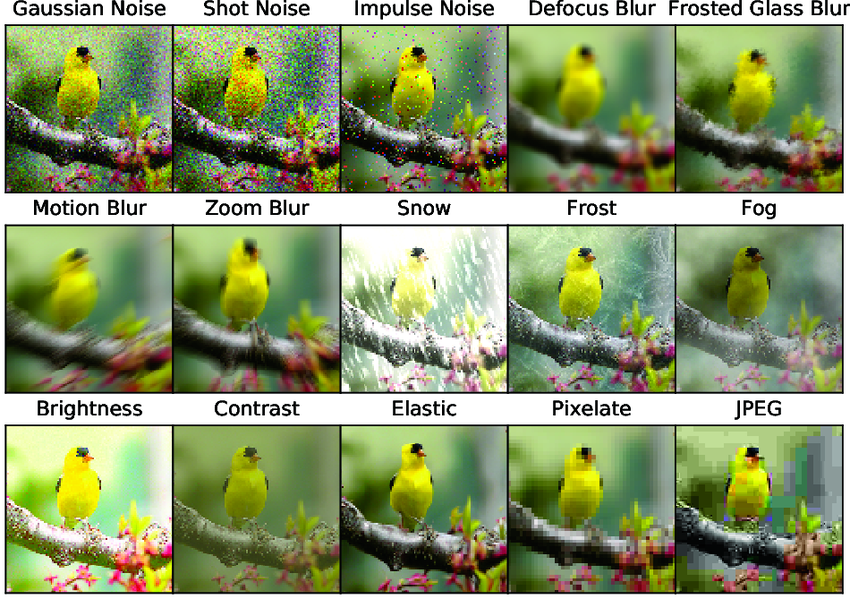
\includegraphics[width=\textwidth,height=0.8\textheight,keepaspectratio]{images/ImageNetC_example.png}
        \end{column}
    \end{columns}
\end{frame}

\begin{frame}{ImageNet-R (Rendition)}
    \begin{columns}
        \begin{column}{0.5\textwidth}
            \begin{itemize}
                \item Valuta il modello su \textbf{immagini stilizzate e artistiche}.
                \item Selezionato un subset di \textbf{200 classi} di ImageNet-1k, reperite via web scraping su Flickr.
                \item Immagini etichettate per stili: \textit{art, cartoon, graffiti, painting, sculpture, toy, origami}, ecc.
                \item Filtro di qualità manuale tramite Amazon Mechanical Turk.
                \item Totale: $\sim$30.000 immagini di test (media 150 per classe).
            \end{itemize}
        \end{column}
        \begin{column}{0.5\textwidth}
            \centering
            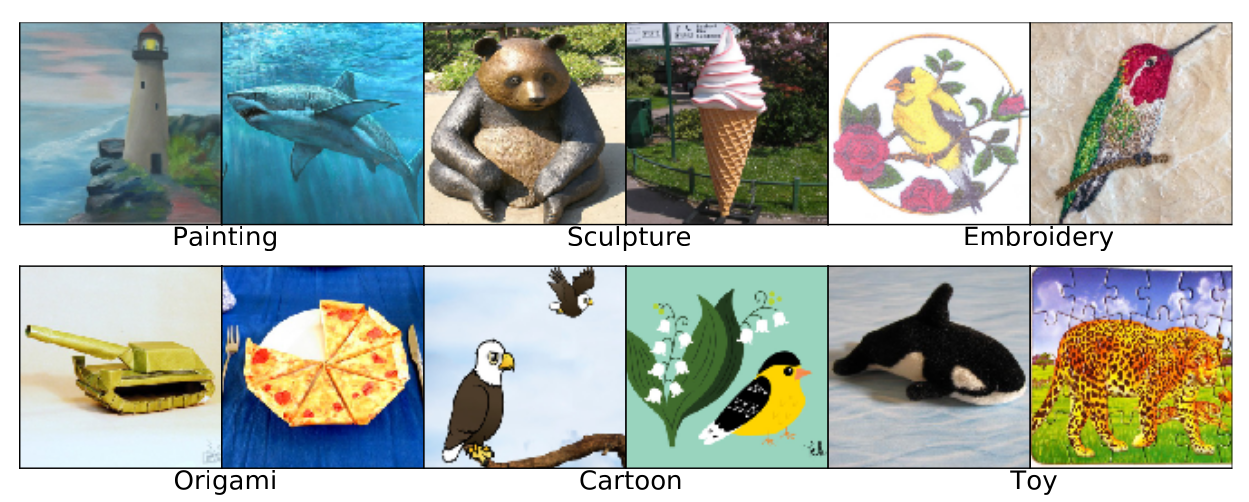
\includegraphics[width=\textwidth,height=0.8\textheight,keepaspectratio]{images/ImageNetR_example.png}
        \end{column}
    \end{columns}
\end{frame}

% --- CAPITOLO 3: IL MODELLO ---
\section{Il Modello: ResNet-50}

\begin{frame}{Reti Neurali Convolutive (CNN)}
    \begin{itemize}
        \item Capaci di sfruttare le \textbf{caratteristiche spaziali} dell'input visivo (es. correlazione tra pixel vicini).
        \item \textbf{Vantaggio}: Riducono drasticamente i parametri rispetto a reti fully-connected usando filtri condivisi (\textit{kernel}).
        \item Architettura base formata da: Strati Convolutivi, Strati di Pooling, Strati Fully-Connected.
    \end{itemize}
    \centering
    \vspace{0.3cm}
    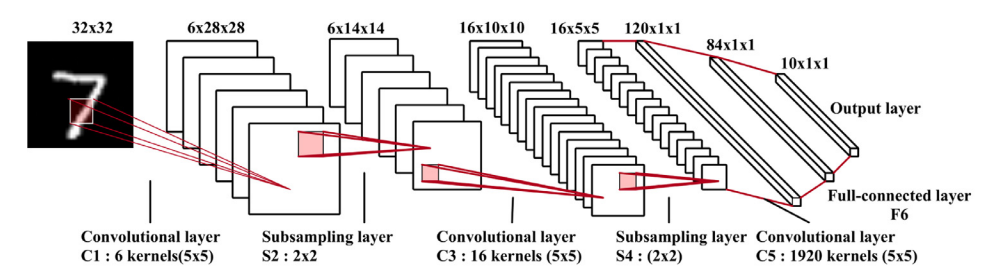
\includegraphics[width=0.7\textwidth]{images/le-net.png}\\
    \textit{\small Esempio storico: Architettura LeNet-5}
\end{frame}

\begin{frame}{Estrazione delle Feature Maps}
    \begin{columns}
        \begin{column}{0.5\textwidth}
            Nei layer convolutivi, il kernel "scorre" sull'immagine estraendo caratteristiche.
            \vspace{0.3cm}
            \begin{itemize}
                \item Un kernel mappa regioni locali.
                \item Viene applicata una funzione di attivazione non lineare.
                \item Layer profondi imparano feature sempre più complesse e astratte.
            \end{itemize}
        \end{column}
        \begin{column}{0.5\textwidth}
            \centering
            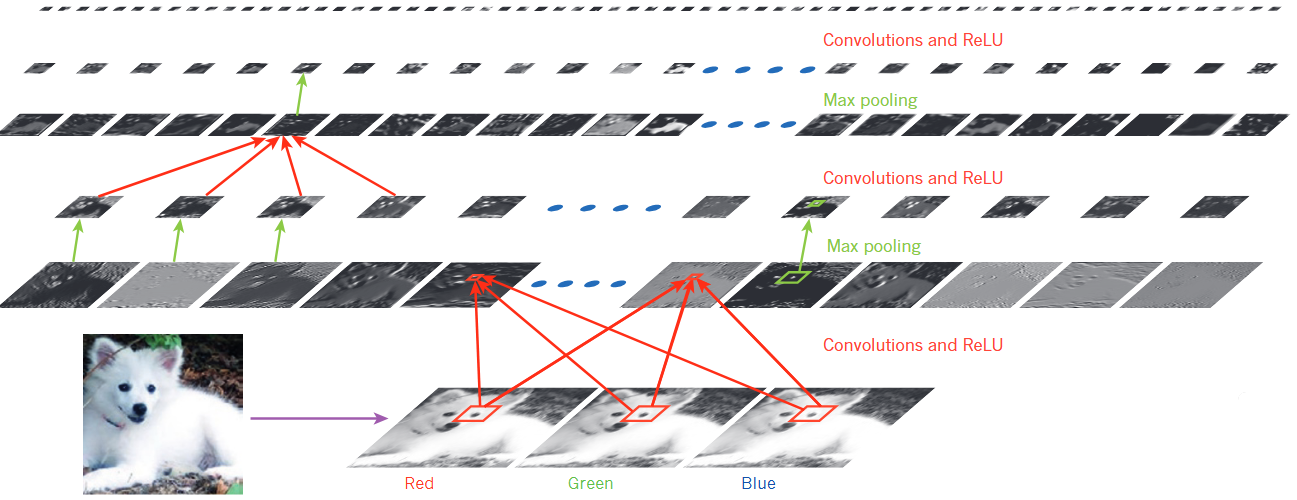
\includegraphics[width=\textwidth,height=0.7\textheight,keepaspectratio]{images/feature maps.png}
        \end{column}
    \end{columns}
\end{frame}

\begin{frame}{Il problema della degradazione e le ResNet}
    \begin{columns}
        \begin{column}{0.5\textwidth}
            \textbf{Problema}: Aumentando i layer, l'accuratezza satura e poi decade (non a causa dell'overfitting).
            \vspace{0.3cm}\\
            \textbf{Soluzione (Reti Residuali)}:
            \begin{itemize}
                \item Apprendimento residuale: impara il mapping $F(x) = H(x) - x$ invece di $H(x)$, dove $H(x)$ è il mapping desiderato.
                \item Uso di \textbf{Identity shortcut connections}: connessioni che saltano uno o più layer, facilitando l'ottimizzazione.
            \end{itemize}
        \end{column}
        \begin{column}{0.5\textwidth}
            \centering
            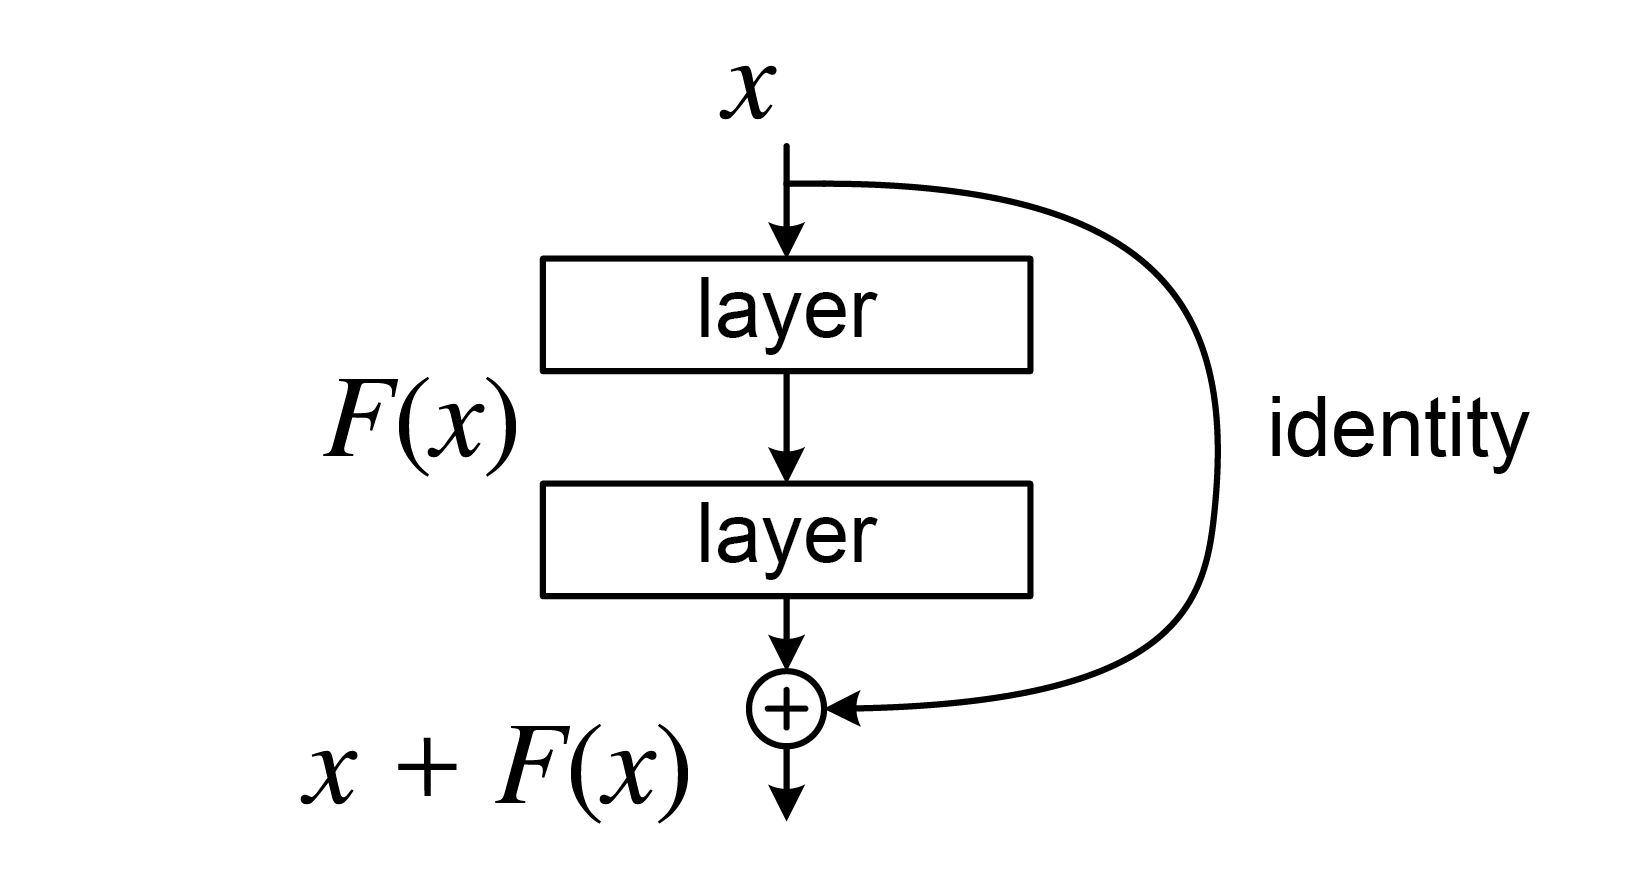
\includegraphics[width=0.8\textwidth]{images/resnet.png}\\
            \vspace{0.2cm}
            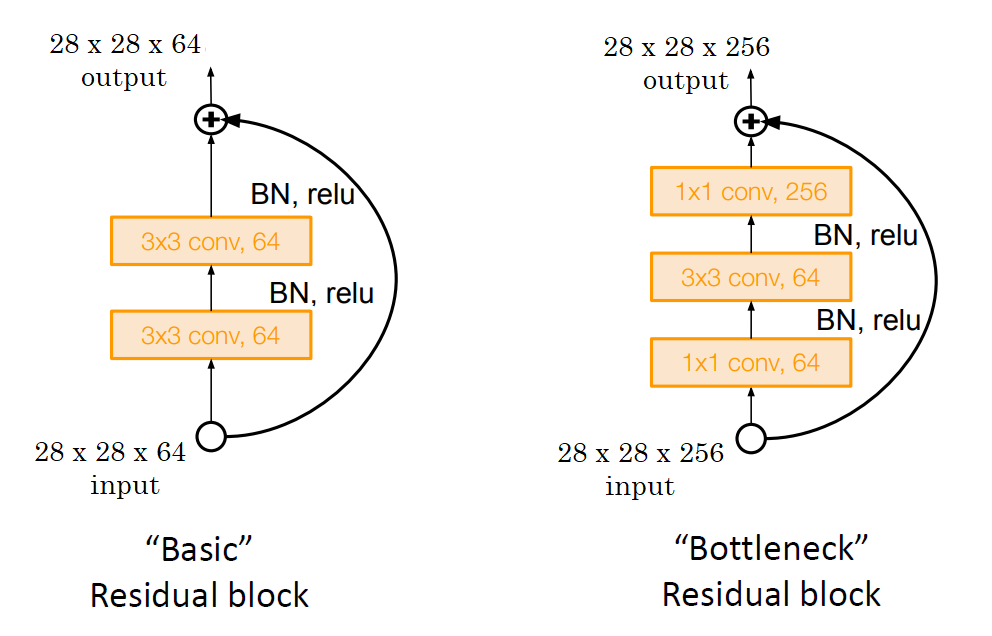
\includegraphics[width=0.8\textwidth]{images/bottleneck.PNG}
        \end{column}
    \end{columns}
\end{frame}

% --- CAPITOLO 4: METODOLOGIA ---
\section{Metodologia}

\begin{frame}{Pipeline di Testing e Preprocessing}
    \begin{itemize}
        \item \textbf{Librerie}: Sviluppo in PyTorch, elaborazione dataset tramite HuggingFace e Arrow per l'efficienza. Evidenze di drift tramite \texttt{Evidently} (Wasserstein) e \texttt{Alibi detect} (MMD).
        \item \textbf{Filtro Dataset}: Per il test su ImageNet-R, ImageNet-1k è stato filtrato mantenendo solo le 200 classi in comune, per garantire un confronto paritario. Mentre ImageNet-R è stato tagliato a 50 immagini per classe.
        \item \textbf{Inferenza}: Uso di \textbf{ResNet-50} con pesi pre-addestrati (senza fine-tuning). Rilevate predizioni ed estratte le feature del penultimo layer (\texttt{avgpool}).
        \item \textbf{Metriche}: Calcolate Accuracy e top-5 Accuracy su 5 ripetizioni con \textit{augmentation stocastica} per stimare gli Intervalli di Confidenza (Test $t$ di Welch).
    \end{itemize}
\end{frame}

\begin{frame}{Le due facce del Drift}
    L'analisi del drift è stata condotta a due livelli:
    \vspace{0.4cm}
    \begin{enumerate}
        \item \textbf{Sulle proprietà visive}: Estrazione di Luminosità, Contrasto RMS, Nitidezza (Sharpness) e medie dei canali RGB (tramite PIL).
        \begin{itemize}
            \item Misurato tramite \textbf{Distanza di Wasserstein} (soglia di drift: $0.1$).
        \end{itemize}
        \vspace{0.3cm}
        \item \textbf{Sulle feature di rete}: Vettori a 2048 dimensioni estratti internamente dal modello.
        \begin{itemize}
            \item Misurato tramite Test MMD (Maximum Mean Discrepancy, drift se p-value $< 0.05$).
        \end{itemize}
    \end{enumerate}
\end{frame}

% --- CAPITOLO 5: RISULTATI - DRIFT ---
\section{Risultati: Misurazione del Drift}

\begin{frame}{Drift Visivo su ImageNet-R}
    \begin{columns}
        \begin{column}{0.4\textwidth}
            La maggior parte delle feature presenta drift rispetto a ImageNet-1k.\\
            \vspace{0.2cm}
            \begin{itemize}
                \item Drift significativo ovunque eccetto che per la \textit{sharpness}.
                \item Alta varianza per la \textit{brightness} (molte immagini artistiche hanno sfondi bianchi).
            \end{itemize}
        \end{column}
        \begin{column}{0.6\textwidth}
            \centering
            
\includegraphics[width=0.7\textwidth]{images/metrics/ImageNet-R/drift_distr_imagenet-1k_vs_imagenet-r.png}
        \end{column}
    \end{columns}
\end{frame}

\begin{frame}{Drift sulle Feature della Rete (MMD)}
    Anche internamente al modello, ImageNet-R genera un forte drift.
    \vspace{0.5cm}
    \begin{table}[]
        \centering
        \begin{tabular}{llll}
        \toprule
        dataset & is\_drift & p\_val & distance \\
        \midrule
        ImageNetR & \textcolor{red}{True} & 0.0000 & 0.0805 \\ 
        \bottomrule
        \end{tabular}
    \end{table}
    \vspace{0.2cm}
    \begin{itemize}
        \item p-value pari a 0 (sotto la soglia 0.05).
        \item Coerente con il drift rilevato visivamente.
    \end{itemize}
\end{frame}
\begin{frame}{ImageNet-C: Drift Visivo - Categoria Blur}
	\begin{columns}

		\begin{column}{0.4\textwidth}
			Valori della distanza di Wasserstein per le feature visive sulle corruzioni di tipo Blur (Motion, Zoom, Defocus, Glass, Frost).\\
		\end{column}
		\begin{column}{0.6\textwidth}
		\begin{figure}
			\centering
			
\includegraphics[width=0.75\textwidth,height=\textheight,keepaspectratio,trim={0 0 0 2cm},clip]{images/metrics/ImageNet-C/severity_curves/imagenet_c_severity_drift_blur.png}
		\end{figure}
		\end{column}
	\end{columns}

\end{frame}

\begin{frame}{ImageNet-C: Drift Visivo - Categoria Blur, esempio: Glass Blur}
    \begin{columns}
        \begin{column}{0.4\textwidth}
            \textbf{Distribuzioni Blur} (\textit{es. Glass Blur}):
            \begin{itemize}
                \item Luminosità e canali colore non presentano variazioni significative.
                \item Il contrasto e la nitidezza subiscono un forte slittamento a causa della fusione dei bordi.
            \end{itemize}
        \end{column}
        \begin{column}{0.6\textwidth}
            \centering
            
\includegraphics[width=\textwidth,height=0.9\textheight,keepaspectratio,trim={0 0 0 0.8cm},clip]{images/metrics/ImageNet-C/distributions_by_corruption/glass_blur.png}
        \end{column}
    \end{columns}
\end{frame}
\begin{frame}{ImageNet-C: Drift Visivo - Categoria Noise}
	\begin{columns}

		\begin{column}{0.4\textwidth}
			Valori della distanza di Wasserstein per le feature visive sulle corruzioni di tipo Noise (Gaussian, Shot, Impulse).\\
		\end{column}
		\begin{column}{0.6\textwidth}
		\begin{figure}
			\centering
			
\includegraphics[width=0.75\textwidth,height=\textheight,keepaspectratio,trim={0 0 0 2cm},clip]{images/metrics/ImageNet-C/severity_curves/imagenet_c_severity_drift_noise.png}
		\end{figure}
		\end{column}
	\end{columns}

\end{frame}

\begin{frame}{ImageNet-C: Drift Visivo - Categoria Noise, esempio: Gaussian Noise}
    \begin{columns}
        \begin{column}{0.4\textwidth}
            \textbf{Distribuzioni Noise} (\textit{es. Gaussian}):
            \begin{itemize}
                \item Il rumore elettronico o termico altera pesantemente le alte frequenze.
                \item La \textit{sharpness} schizza a valori elevatissimi (distanza di Wasserstein $> 4$) poiché il rumore viene scambiato per micro-bordi.
            \end{itemize}
        \end{column}
        \begin{column}{0.6\textwidth}
            \centering
            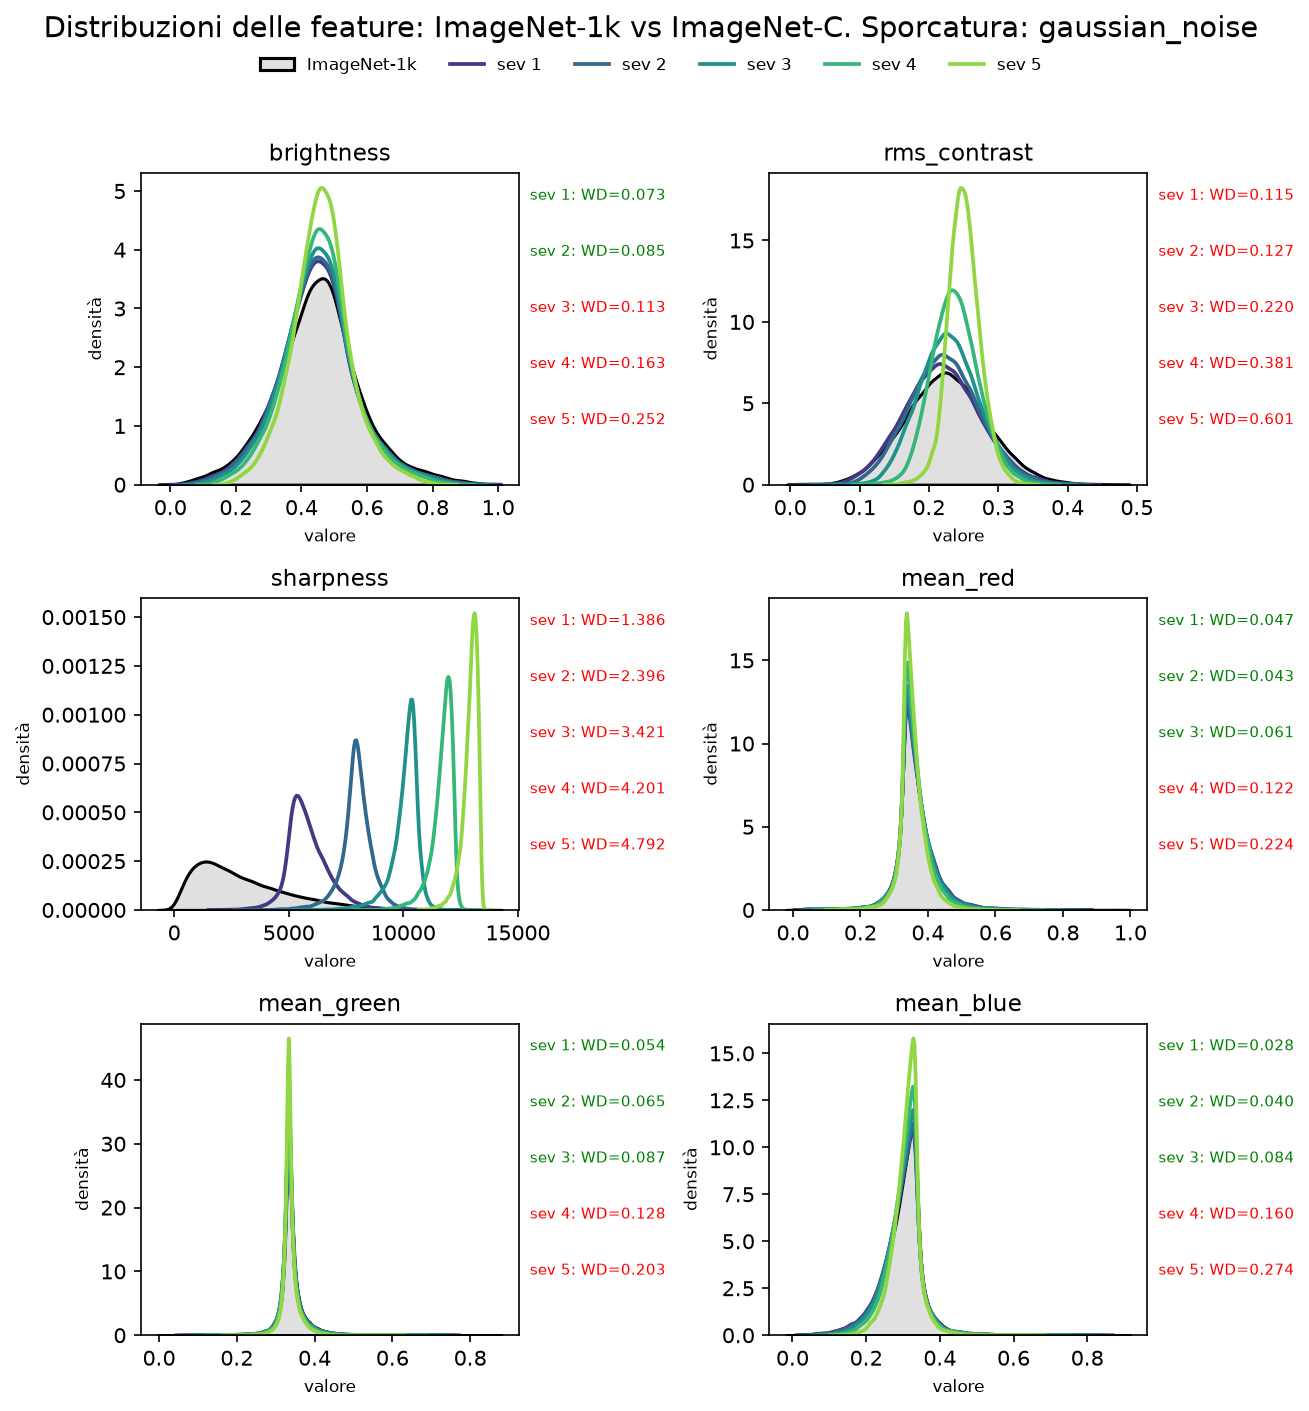
\includegraphics[width=\textwidth,height=0.9\textheight,keepaspectratio,trim={0 0 0 0.8cm},clip]{images/metrics/ImageNet-C/distributions_by_corruption/gaussian_noise.png}
        \end{column}
    \end{columns}
\end{frame}
\begin{frame}{ImageNet-C: Drift Visivo - Categoria Weather}
	\begin{columns}
		\begin{column}{0.4\textwidth}
			Valori della distanza di Wasserstein per le feature visive sulle corruzioni di tipo Weather (Fog, Snow, Rain, Brightness).\\
		\end{column}
		\begin{column}{0.6\textwidth}
		\begin{figure}
			\centering
			
\includegraphics[width=0.75\textwidth,height=\textheight,keepaspectratio,trim={0 0 0 2cm},clip]{images/metrics/ImageNet-C/severity_curves/imagenet_c_severity_drift_weather.png}
		\end{figure}
		\end{column}
	\end{columns}
\end{frame}
\begin{frame}{ImageNet-C: Drift Visivo - Categoria Weather, esempio: Fog}
    \begin{columns}
        \begin{column}{0.4\textwidth}
            \textbf{Distribuzioni Weather} (\textit{es. Fog}):
            \begin{itemize}
                \item La nebbia appiattisce il contrasto comprimendo le distribuzioni verso un grigio uniforme.
                \item I canali colore tendono a convergere verso valori medi simili, riducendo la saturazione.
                \item La nitidezza cala drasticamente a causa della fusione dei bordi.
            \end{itemize}
        \end{column}
        \begin{column}{0.6\textwidth}
            \centering
            
\includegraphics[width=\textwidth,height=0.9\textheight,keepaspectratio,trim={0 0 0 0.8cm},clip]{images/metrics/ImageNet-C/distributions_by_corruption/fog.png}
        \end{column}
    \end{columns}
\end{frame}

\begin{frame}{ImageNet-C: Drift Visivo - Categoria Digital}
	\begin{columns}
		\begin{column}{0.4\textwidth}
			Valori della distanza di Wasserstein per le feature visive sulle corruzioni di tipo Digital (Contrast, Elastic Transform, JPEG Compression).\\
		\end{column}
		\begin{column}{0.6\textwidth}
		\begin{figure}
			\centering
			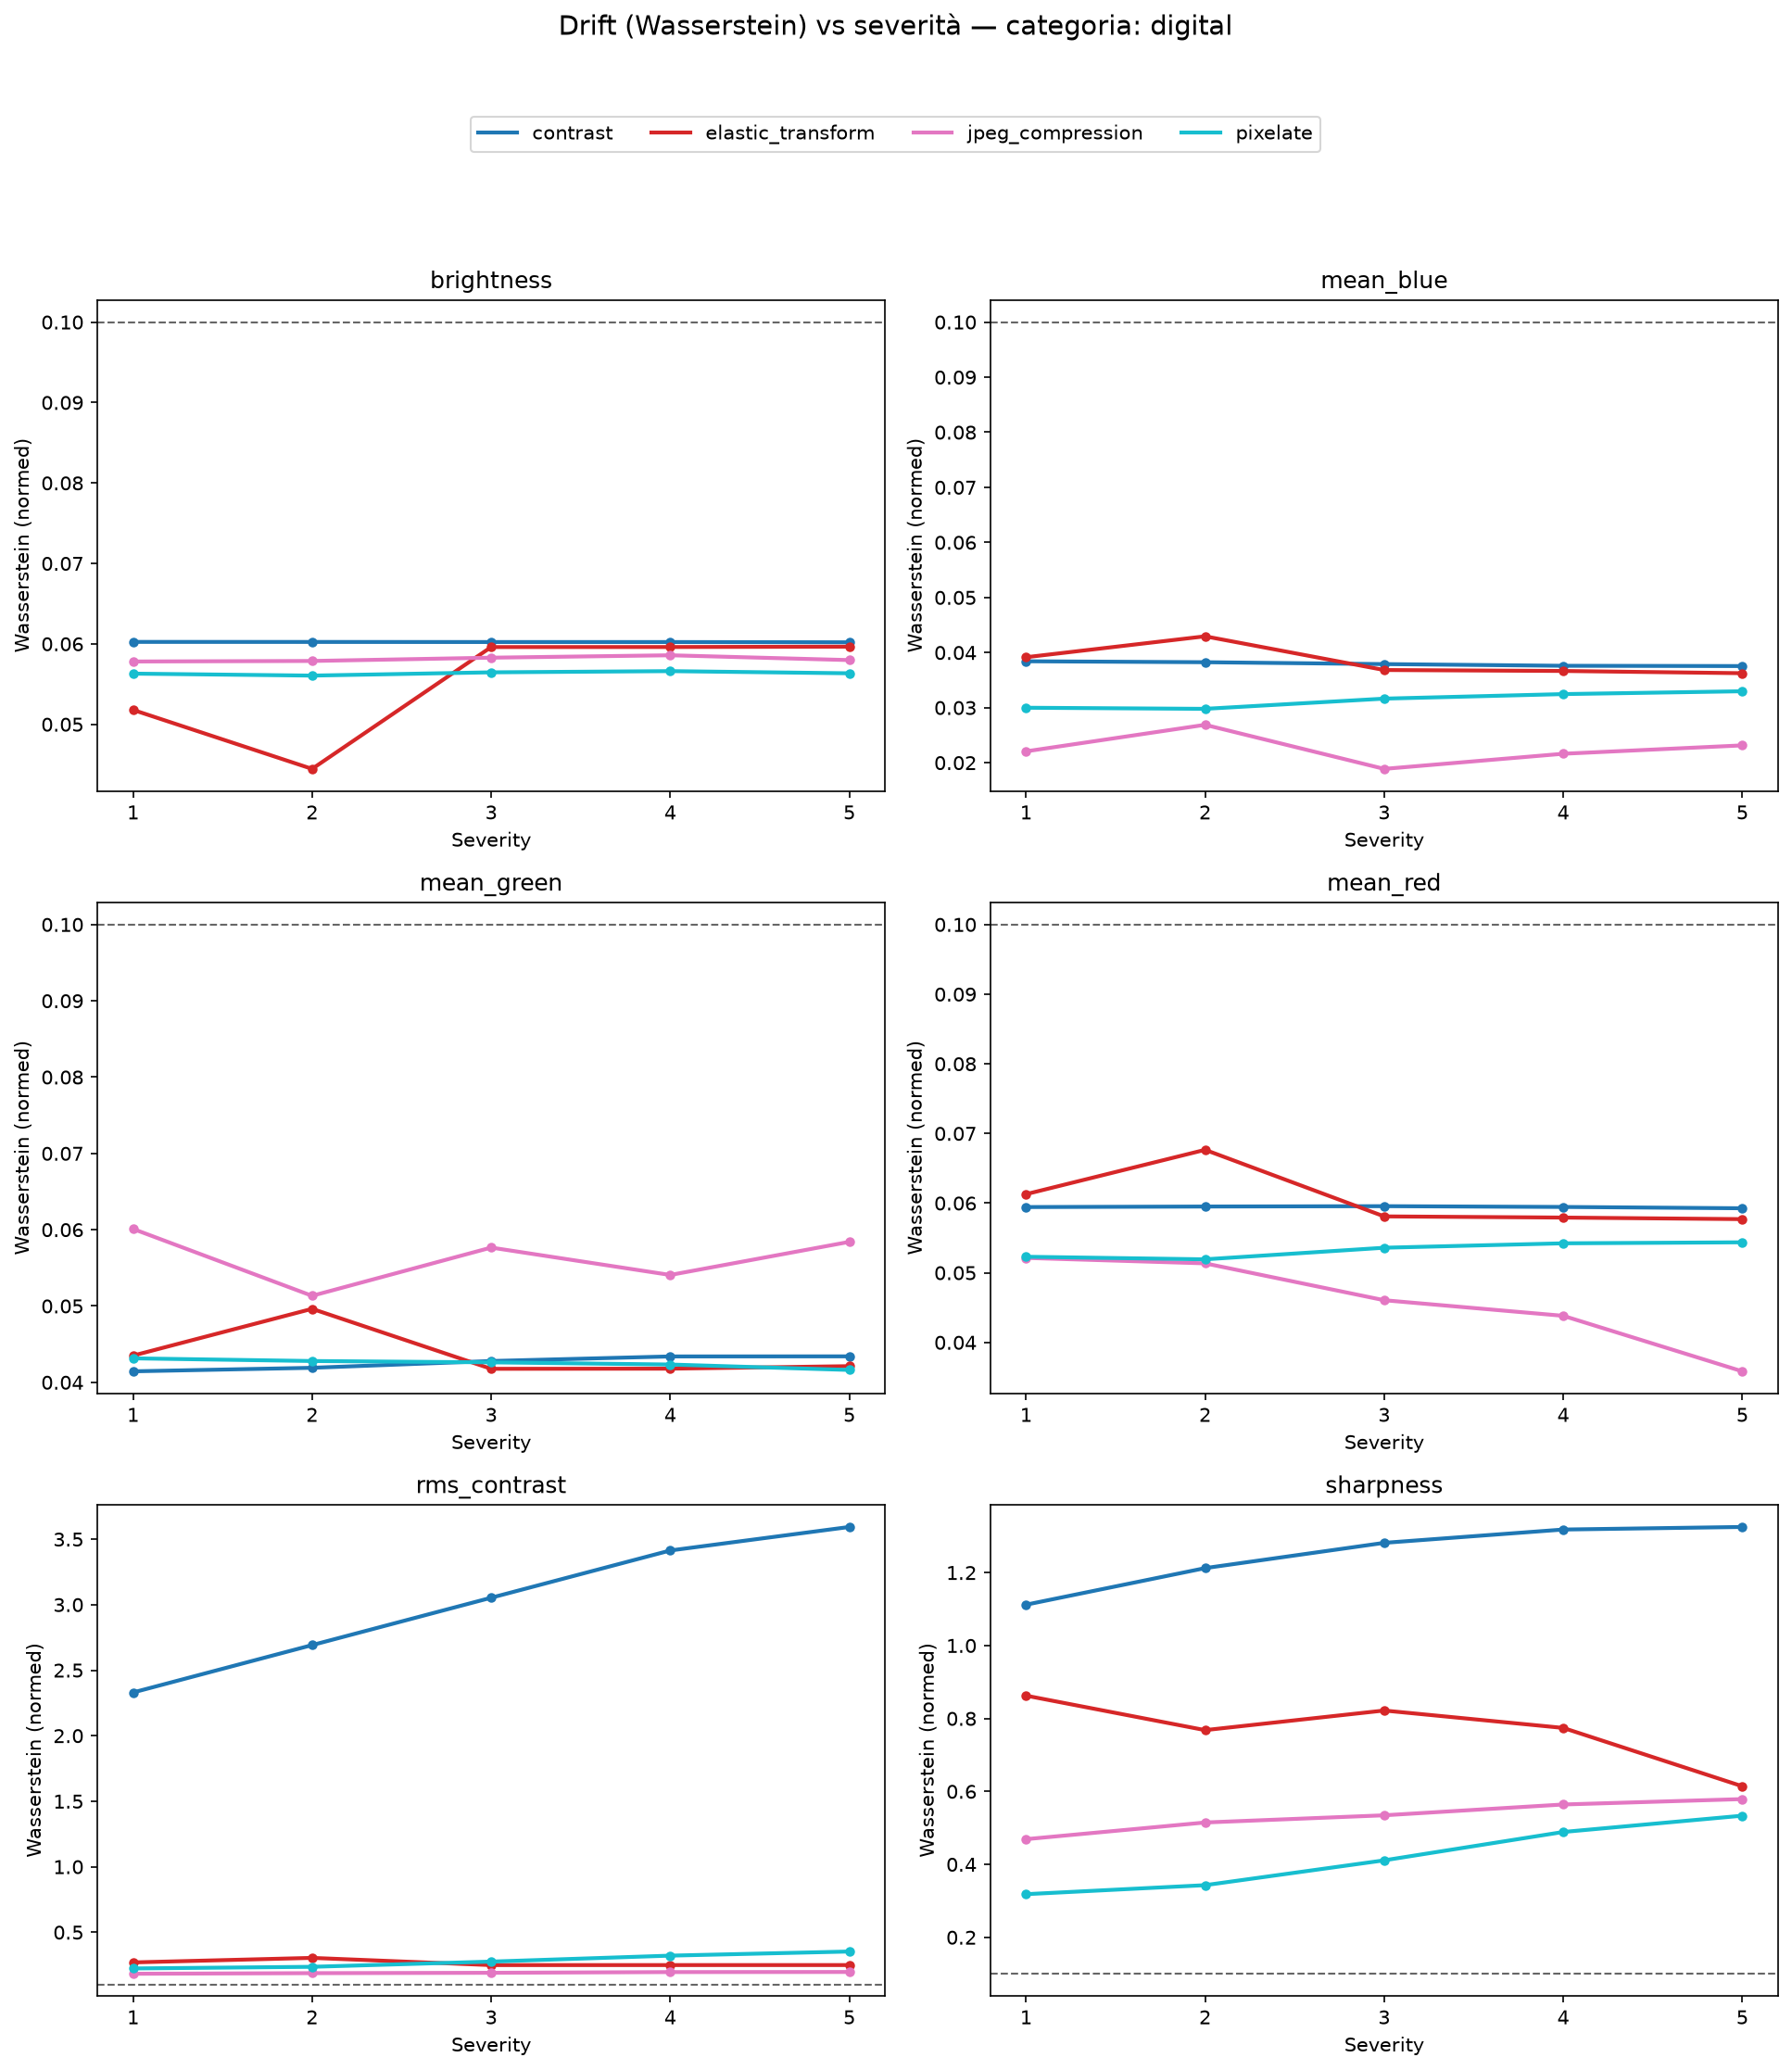
\includegraphics[width=0.75\textwidth,height=\textheight,keepaspectratio,trim={0 0 0 2cm},clip]{images/metrics/ImageNet-C/severity_curves/imagenet_c_severity_drift_digital.png}
		\end{figure}
		\end{column}
	\end{columns}
\end{frame}
\begin{frame}{ImageNet-C: Drift Visivo - Categoria Digital, esempio: Contrast}
    \begin{columns}
        \begin{column}{0.4\textwidth}
            \textbf{Distribuzioni Digital} (\textit{es. Contrast}):
            \begin{itemize}
                \item La manipolazione diretta del contrasto sposta radicalmente la metrica RMS contrast.
                \item Le medie dei canali colore rimangono stranamente stabili nonostante la forte alterazione visiva.
            \end{itemize}
        \end{column}
        \begin{column}{0.6\textwidth}
            \centering
            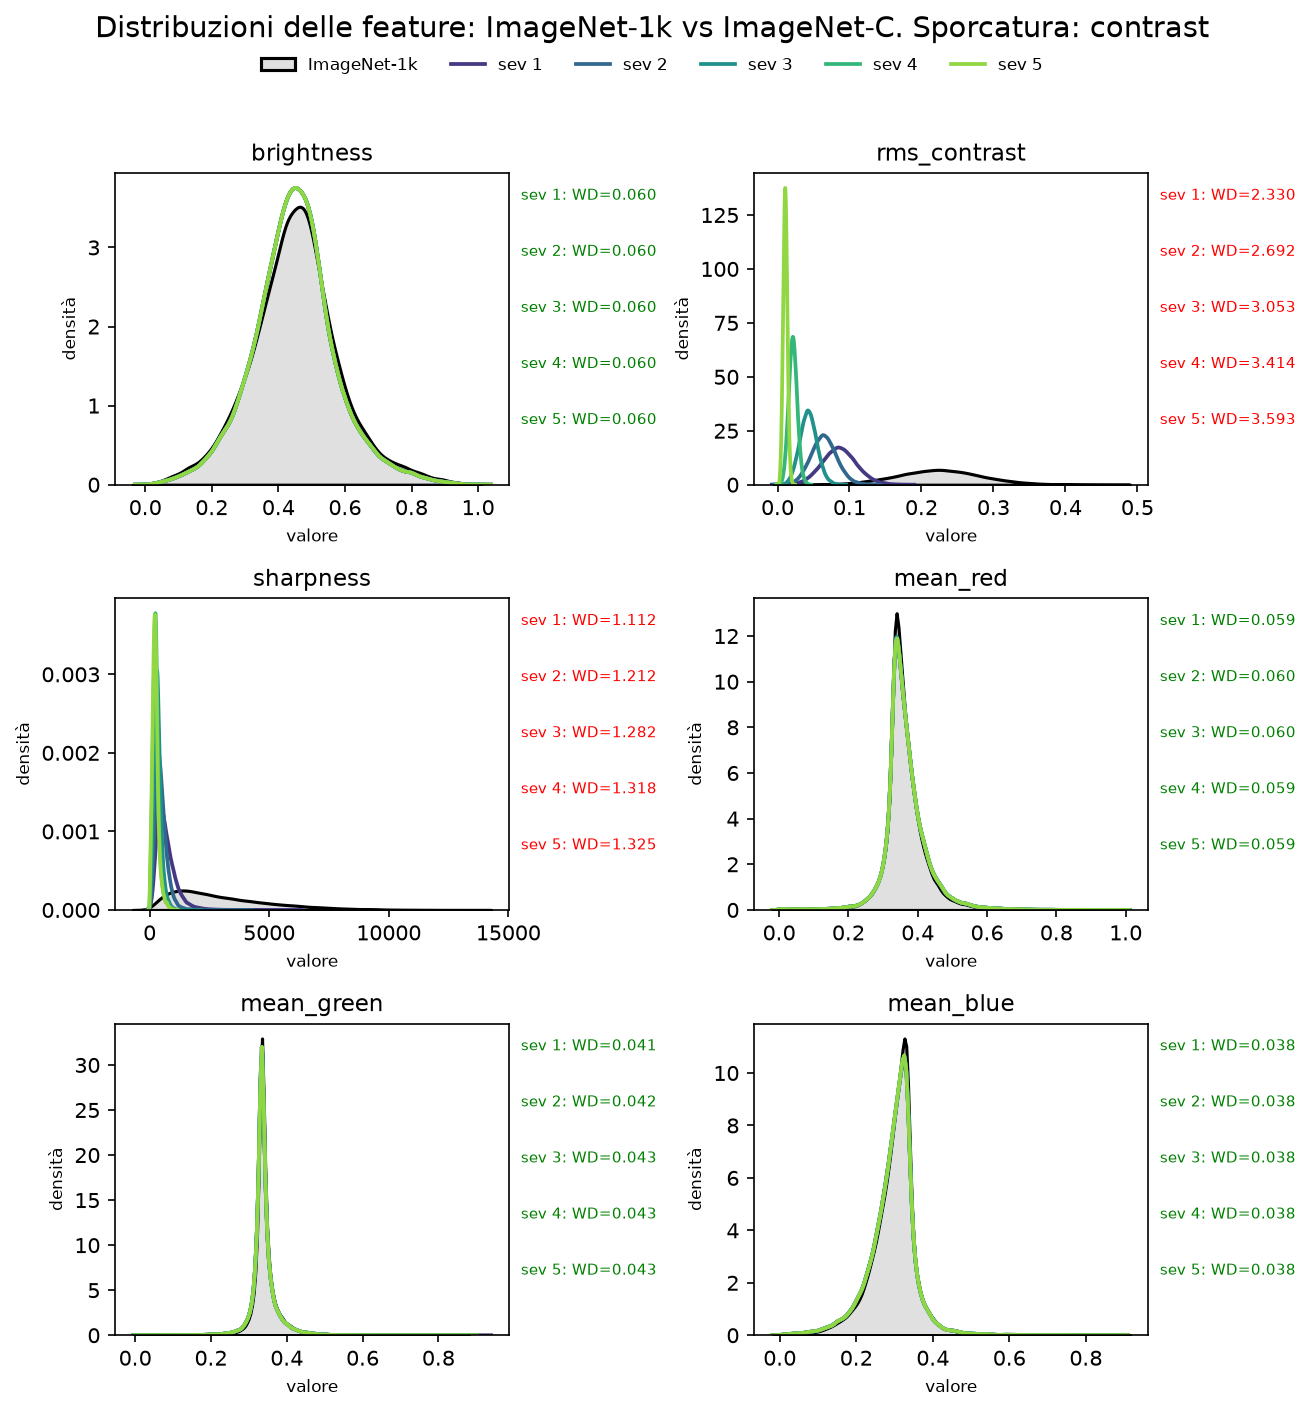
\includegraphics[width=\textwidth,height=0.9\textheight,keepaspectratio,trim={0 0 0 0.8cm},clip]{images/metrics/ImageNet-C/distributions_by_corruption/contrast.png}
        \end{column}
    \end{columns}
\end{frame}

\begin{frame}{Drift Feature Rete (MMD) vs Drift Visivo su ImageNet-C}
    \textbf{Discrepanza interessante:}
    \vspace{0.2cm}
    \begin{itemize}
        \item \textbf{Digital \& Noise}: Visivamente, il drift per le feature \textit{sharpness} e \textit{contrasto} è sempre alto, anche a severità 1 e 2.
        \item \textbf{Reti Neurali}: Il test MMD \textbf{non} rileva drift sulle feature di \texttt{avgpool} per i primi livelli di severità per corruzioni come \textit{Contrast}, \textit{Motion Blur}, \textit{Brightness}, o \textit{Gaussian Noise}. Per \textit{JPEG\_compression}, non rileva drift a nessuna severità.
        \item \textbf{Significato}: Le caratteristiche utilizzate dalla rete per classificare sono fondamentalmente diverse da quelle estratte staticamente dai pixel dell'immagine.
    \end{itemize}
\end{frame}

% --- CAPITOLO 6: RISULTATI - PERFORMANCE ---
\section{Risultati: Analisi delle Performance}

\begin{frame}{Impatto di ImageNet-R sulle Metriche}
    \begin{table}[]
        \centering
        \begin{tabular}{lcccc}
        \hline
        \textbf{Metric} & \textbf{IN-1k} & \textbf{IN-R} & \textbf{Delta} & \textbf{Sig.} \\
        \hline
        Accuracy            & 84.33\% & 30.34\% & 53.98\% & YES \\
        Top-5 accuracy      & 96.35\% & 45.72\% & 50.63\% & YES \\
        \hline
        \end{tabular}
    \end{table}
    \vspace{0.3cm}
    \begin{itemize}
        \item Tutte le metriche calano drasticamente e in modo statisticamente significativo.
        \item \textcolor{red}{\textbf{-53.9\% di Accuratezza}}: Il Covariate Shift introdotto da un cambio di stile visivo (arte, cartoni, ecc.) devasta la capacità di generalizzazione di ResNet-50.
    \end{itemize}
\end{frame}

\begin{frame}{Degradazione su ImageNet-C: Blur}
    \begin{columns}
        \begin{column}{0.4\textwidth}
            \begin{itemize}
                \item La degradazione cresce all'aumentare della severità per tutti i tipi di blur.
                \item \textbf{Glass Blur} ha un crollo drastico non lineare (AUC di Robustness bassissima: 0.369), portando l'accuratezza ben sotto il 10\% a severità 5.
                \item \textbf{Zoom Blur} mostra il comportamento di degrado più lineare ($R^2 = 0.99$).
            \end{itemize}
        \end{column}
        \begin{column}{0.6\textwidth}
            \centering
            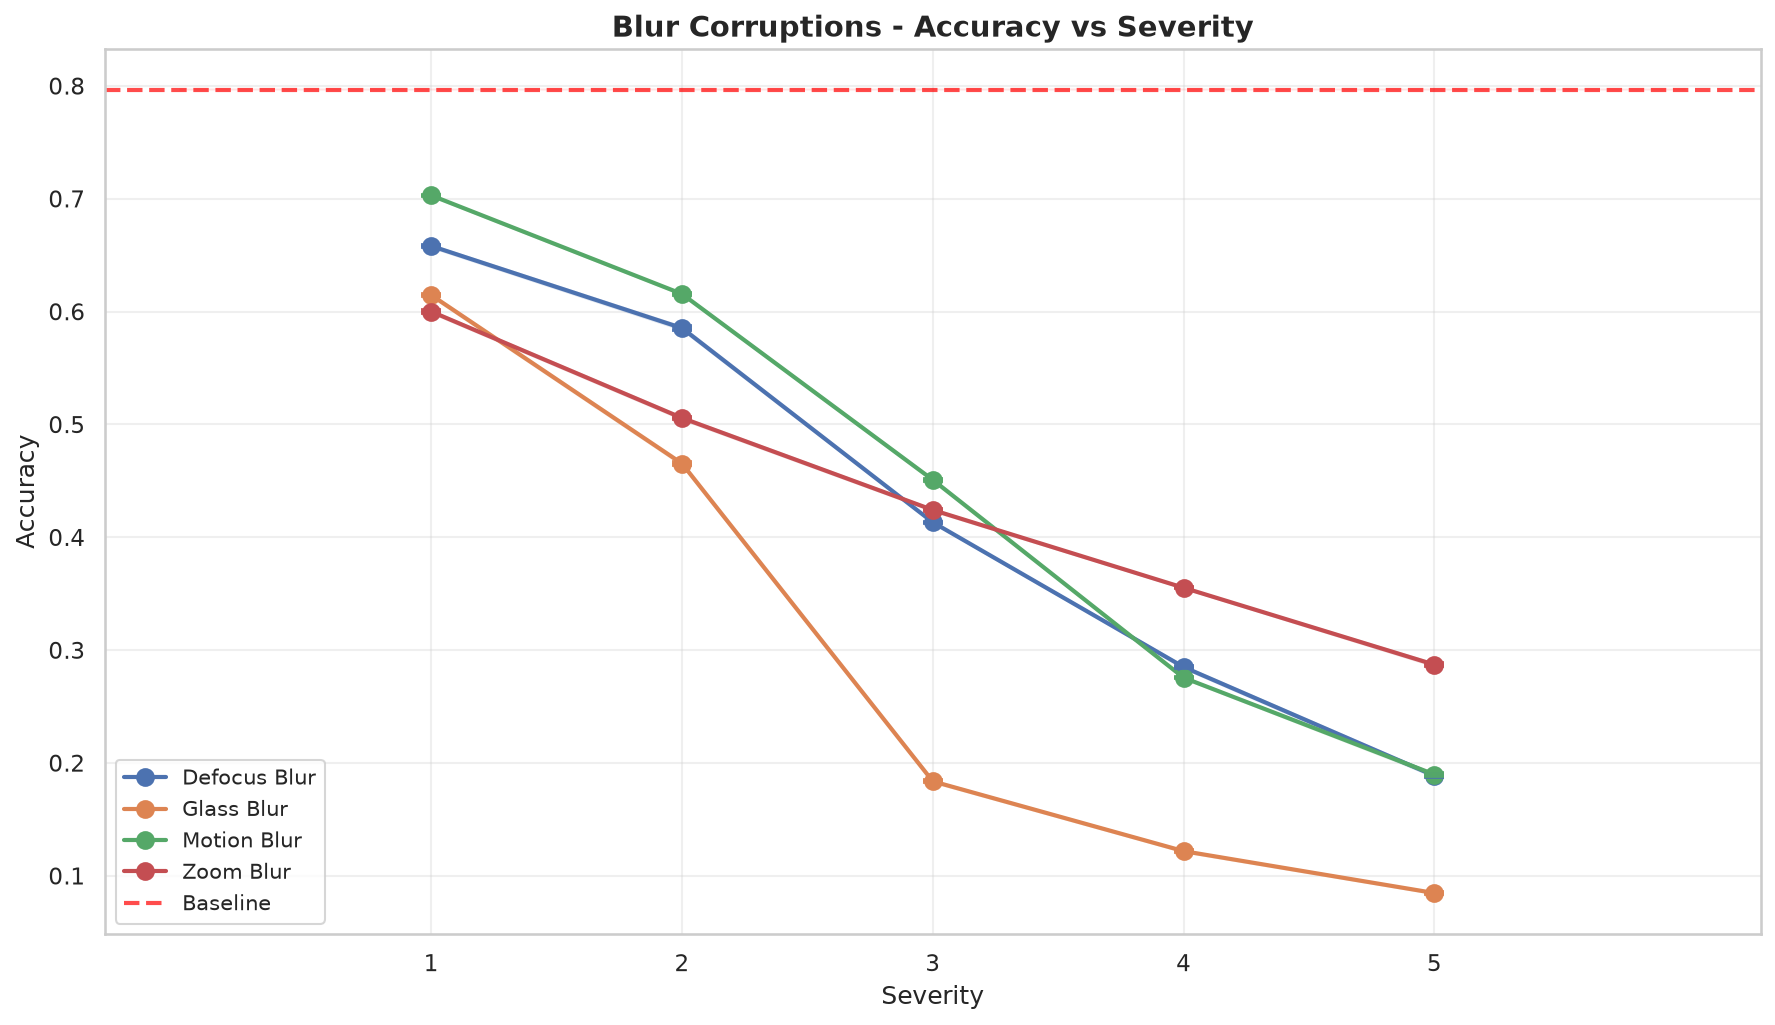
\includegraphics[width=\textwidth]{images/plot_metrics/categories/blur_accuracy.png}
        \end{column}
    \end{columns}
\end{frame}

\begin{frame}{Degradazione su ImageNet-C: Noise}
    \begin{columns}
        \begin{column}{0.4\textwidth}
            \begin{itemize}
                \item L'impatto del rumore è quasi lineare e gravissimo.
                \item Ai primissimi livelli (1-2) il modello regge parzialmente (coerentemente con l'assenza di drift MMD a quei livelli).
                \item A severità 5 l'accuratezza crolla a $\sim 10\%$.
                \item \textbf{Impulse noise} risulta il peggiore della categoria (AUC Robustness: 0.482).
            \end{itemize}
        \end{column}
        \begin{column}{0.6\textwidth}
            \centering
            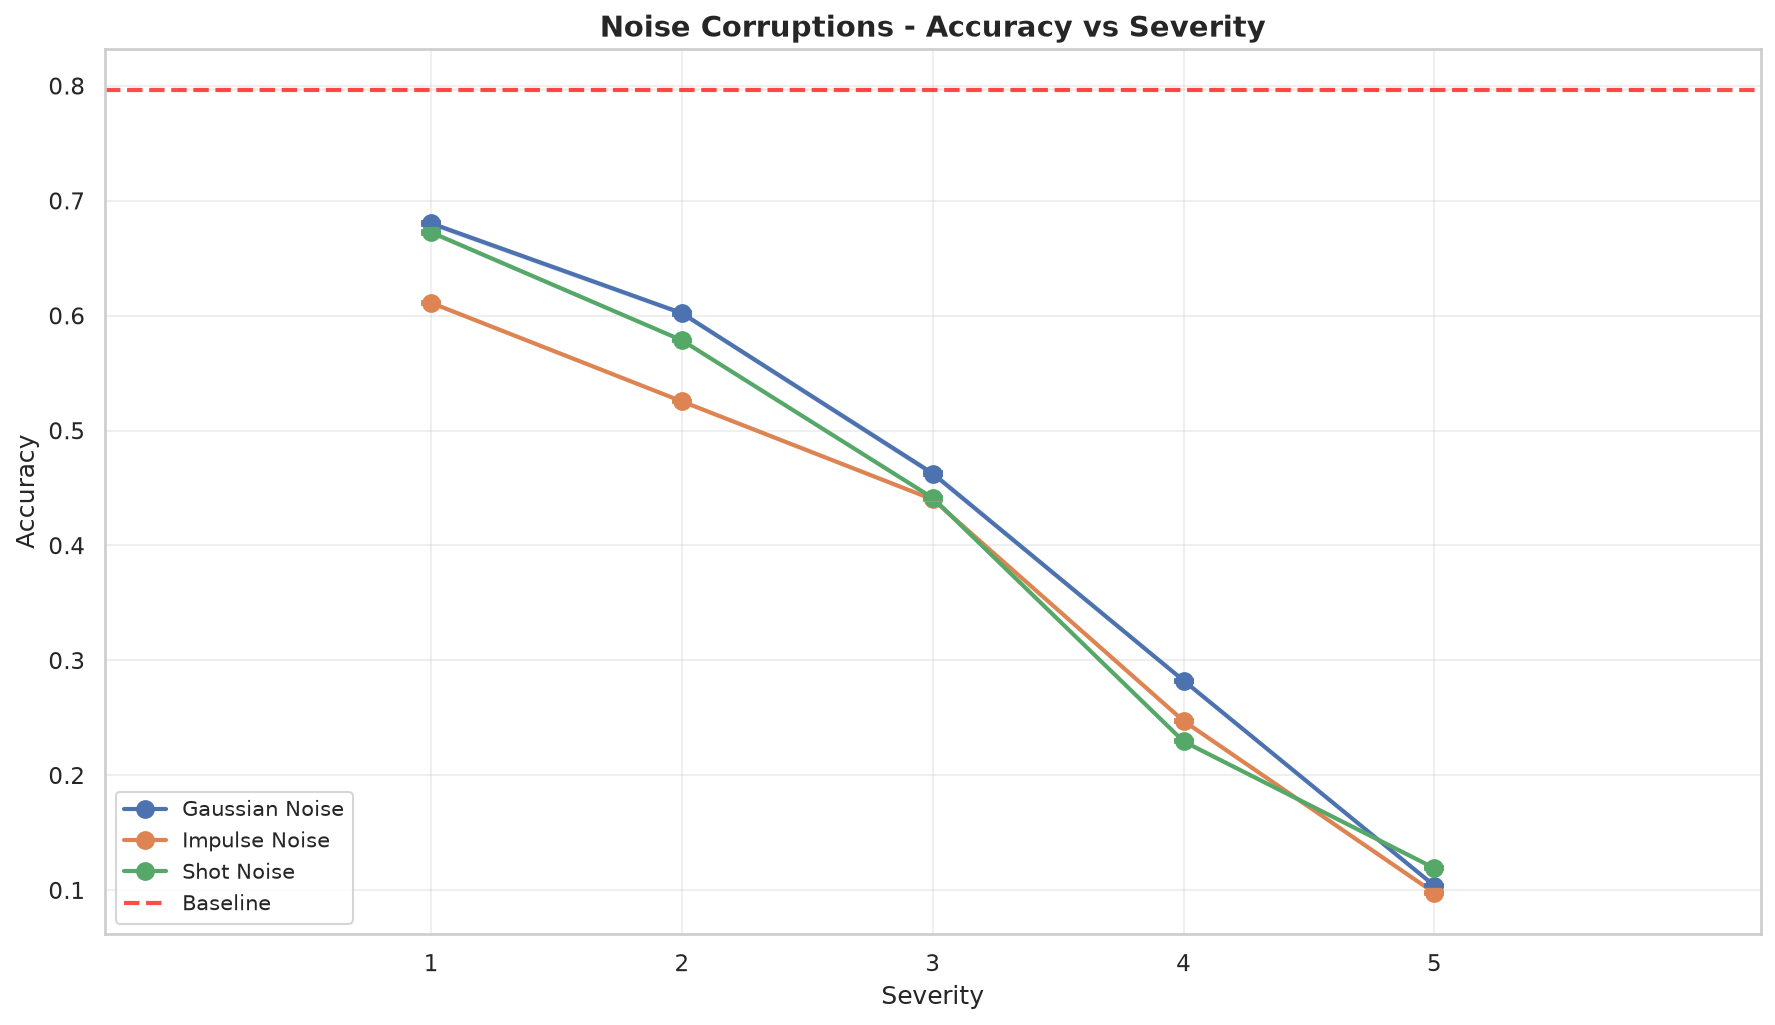
\includegraphics[width=\textwidth]{images/plot_metrics/categories/noise_accuracy.png}
        \end{column}
    \end{columns}
\end{frame}

\begin{frame}{Degradazione su ImageNet-C: Digital}
    \begin{columns}
        \begin{column}{0.4\textwidth}
            \begin{itemize}
                \item Categoria con le performance mediamente più alte.
                \item \textbf{JPEG} e \textbf{Contrast} mantengono accuratezze relativamente buone (AUC Robustness $>$ 0.73), il che si allinea perfettamente con l'assenza di drift MMD sulle feature interne a basse/medie severità.
                \item \textbf{Elastic Transform} fa eccezione: dopo un andamento irregolare crolla precipitosamente a severità 5.
            \end{itemize}
        \end{column}
        \begin{column}{0.6\textwidth}
            \centering
            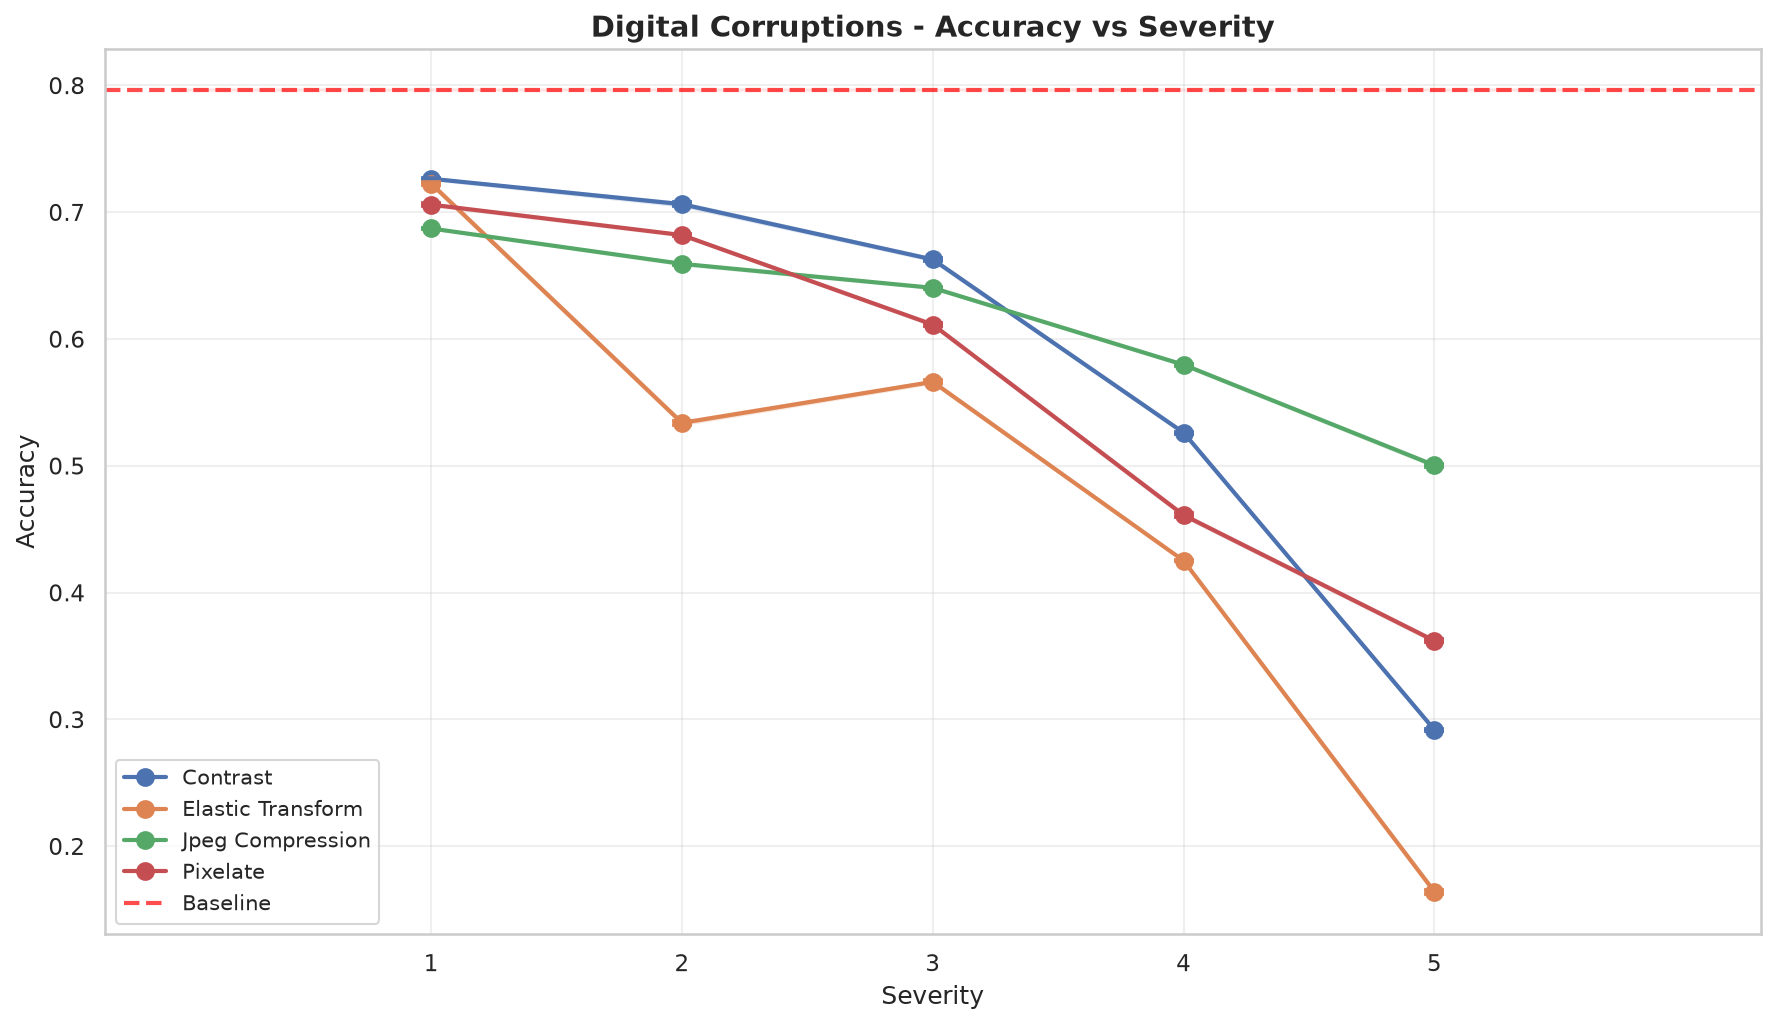
\includegraphics[width=\textwidth]{images/plot_metrics/categories/digital_accuracy.png}
        \end{column}
    \end{columns}
\end{frame}

\begin{frame}{Degradazione su ImageNet-C: Weather}
    \begin{columns}
        \begin{column}{0.4\textwidth}
            \begin{itemize}
                \item Varianza notevole tra le diverse condizioni atmosferiche.
                \item \textbf{Brightness} non impatta quasi per nulla il modello, mantenendo un'accuratezza altissima (AUC Robustness: 0.899).
                \item Anche \textbf{Fog} (nebbia) si mantiene moderatamente robusta.
                \item Al contrario, \textbf{Frost} e \textbf{Snow} distruggono le performance (AUC Robustness $\sim$ 0.50-0.57), probabilmente perché introducono artefatti fisici complessi (cristalli e occlusione) anziché soli cambi cromatici.
            \end{itemize}
        \end{column}
        \begin{column}{0.6\textwidth}
            \centering
            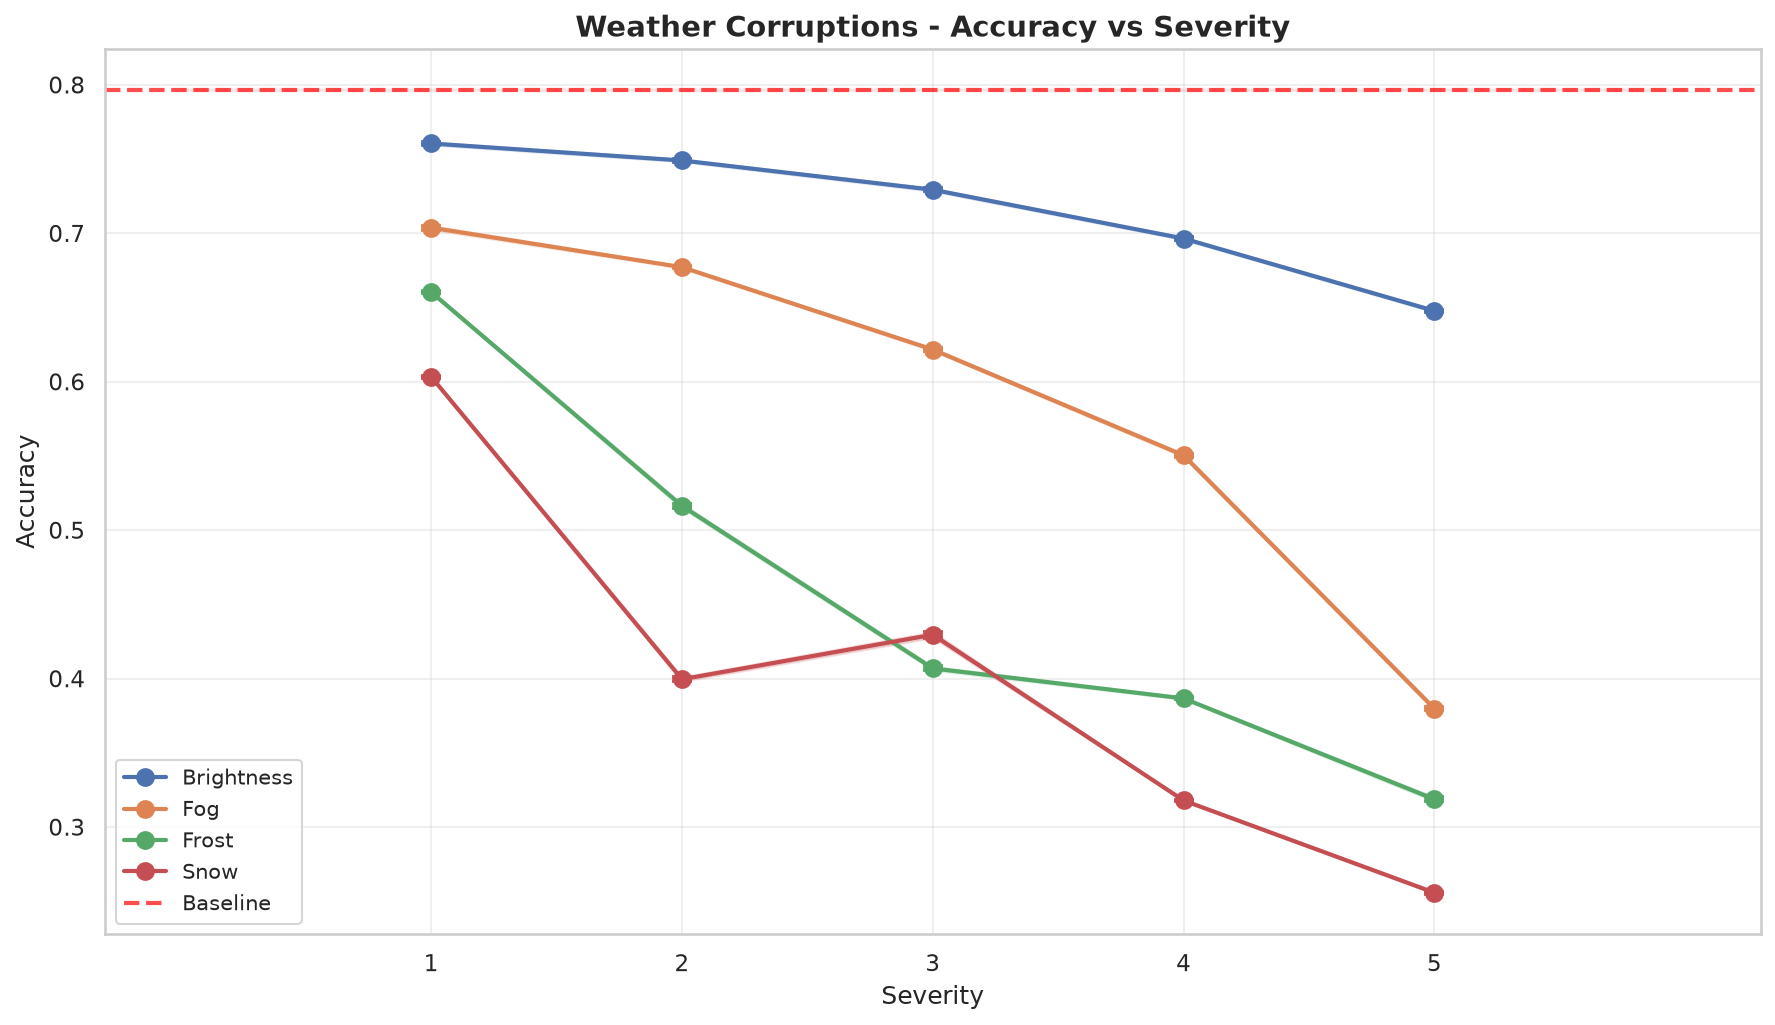
\includegraphics[width=\textwidth]{images/plot_metrics/categories/weather_accuracy.png}
        \end{column}
    \end{columns}
\end{frame}

% --- CAPITOLO 7: CONCLUSIONI ---
\section{Conclusioni e Sviluppi}

\begin{frame}{Conclusioni: Drift e Correlazioni}
    \begin{enumerate}
        \item \textbf{Disaccoppiamento Visivo-Rete}: Non esiste una forte correlazione tra il drift calcolato sui pixel "grezzi" (Wasserstein) e il drift interno al modello (MMD). La rete usa logiche e feature molto diverse da quelle misurabili dall'occhio umano.
        \item \textbf{Correlazione MMD-Performance}: Esiste invece una forte correlazione tra il rilevamento del drift MMD sulle feature di ResNet-50 e l'effettivo calo dell'accuratezza in fase di test.
    \end{enumerate}
\end{frame}

\begin{frame}{Conclusioni: ImageNet-R vs ImageNet-C}
    \textbf{Confronto di impatto globale}:
    \begin{itemize}
        \item A basse severità (1-2), il rumore e le corruzioni fisiche (ImageNet-C) generano un danno nettamente minore rispetto al cambio di stile artistico di ImageNet-R.
        \item Solo ai livelli estremi (severità 4 e 5), le corruzioni fisiche/digitali arrivano a penalizzare il modello in modo più severo (sotto al 30\% di accuratezza).
        \item \textbf{Verdetto finale}: Il covariate shift causato da una variazione concettuale/stilistica (ImageNet-R) è strutturalmente il più difficile da gestire per una CNN addestrata su foto standard, battuto solo da artefatti e degradazioni visive severissime.
    \end{itemize}
\end{frame}

\begin{frame}{Sviluppi Futuri}
    Possibili evoluzioni del progetto includono:
    \begin{itemize}
        \item \textbf{Drift Temporale}: Analizzare ImageNet-V2, dataset campionato successivamente ma con logiche identiche a ImageNet originale, per testare la riproducibilità temporale e il temporal shift.
        \item \textbf{Altri Shift}: Ripetere l'analisi introducendo \textit{Prior Probability Shift} o \textit{Concept Shift}.
        \item \textbf{Architetture Alternative}: Valutare se modelli concettualmente diversi mostrino una robustezza superiore o diversa rispetto alle CNN in presenza dello stesso drift.
    \end{itemize}
\end{frame}

\begin{frame}
    \centering
    \Huge
    Grazie per l'attenzione!
\end{frame}

\end{document}